\documentclass[]{article}
\usepackage{lmodern}
\usepackage{amssymb,amsmath}
\usepackage{ifxetex,ifluatex}
\usepackage{fixltx2e} % provides \textsubscript
\ifnum 0\ifxetex 1\fi\ifluatex 1\fi=0 % if pdftex
  \usepackage[T1]{fontenc}
  \usepackage[utf8]{inputenc}
\else % if luatex or xelatex
  \ifxetex
    \usepackage{mathspec}
  \else
    \usepackage{fontspec}
  \fi
  \defaultfontfeatures{Ligatures=TeX,Scale=MatchLowercase}
\fi
% use upquote if available, for straight quotes in verbatim environments
\IfFileExists{upquote.sty}{\usepackage{upquote}}{}
% use microtype if available
\IfFileExists{microtype.sty}{%
\usepackage{microtype}
\UseMicrotypeSet[protrusion]{basicmath} % disable protrusion for tt fonts
}{}
\usepackage[margin=1in]{geometry}
\usepackage{hyperref}
\hypersetup{unicode=true,
            pdftitle={Grady Lab PostgreSQL Manual},
            pdfauthor={Sean Maden},
            pdfborder={0 0 0},
            breaklinks=true}
\urlstyle{same}  % don't use monospace font for urls
\usepackage{color}
\usepackage{fancyvrb}
\newcommand{\VerbBar}{|}
\newcommand{\VERB}{\Verb[commandchars=\\\{\}]}
\DefineVerbatimEnvironment{Highlighting}{Verbatim}{commandchars=\\\{\}}
% Add ',fontsize=\small' for more characters per line
\usepackage{framed}
\definecolor{shadecolor}{RGB}{248,248,248}
\newenvironment{Shaded}{\begin{snugshade}}{\end{snugshade}}
\newcommand{\KeywordTok}[1]{\textcolor[rgb]{0.13,0.29,0.53}{\textbf{{#1}}}}
\newcommand{\DataTypeTok}[1]{\textcolor[rgb]{0.13,0.29,0.53}{{#1}}}
\newcommand{\DecValTok}[1]{\textcolor[rgb]{0.00,0.00,0.81}{{#1}}}
\newcommand{\BaseNTok}[1]{\textcolor[rgb]{0.00,0.00,0.81}{{#1}}}
\newcommand{\FloatTok}[1]{\textcolor[rgb]{0.00,0.00,0.81}{{#1}}}
\newcommand{\ConstantTok}[1]{\textcolor[rgb]{0.00,0.00,0.00}{{#1}}}
\newcommand{\CharTok}[1]{\textcolor[rgb]{0.31,0.60,0.02}{{#1}}}
\newcommand{\SpecialCharTok}[1]{\textcolor[rgb]{0.00,0.00,0.00}{{#1}}}
\newcommand{\StringTok}[1]{\textcolor[rgb]{0.31,0.60,0.02}{{#1}}}
\newcommand{\VerbatimStringTok}[1]{\textcolor[rgb]{0.31,0.60,0.02}{{#1}}}
\newcommand{\SpecialStringTok}[1]{\textcolor[rgb]{0.31,0.60,0.02}{{#1}}}
\newcommand{\ImportTok}[1]{{#1}}
\newcommand{\CommentTok}[1]{\textcolor[rgb]{0.56,0.35,0.01}{\textit{{#1}}}}
\newcommand{\DocumentationTok}[1]{\textcolor[rgb]{0.56,0.35,0.01}{\textbf{\textit{{#1}}}}}
\newcommand{\AnnotationTok}[1]{\textcolor[rgb]{0.56,0.35,0.01}{\textbf{\textit{{#1}}}}}
\newcommand{\CommentVarTok}[1]{\textcolor[rgb]{0.56,0.35,0.01}{\textbf{\textit{{#1}}}}}
\newcommand{\OtherTok}[1]{\textcolor[rgb]{0.56,0.35,0.01}{{#1}}}
\newcommand{\FunctionTok}[1]{\textcolor[rgb]{0.00,0.00,0.00}{{#1}}}
\newcommand{\VariableTok}[1]{\textcolor[rgb]{0.00,0.00,0.00}{{#1}}}
\newcommand{\ControlFlowTok}[1]{\textcolor[rgb]{0.13,0.29,0.53}{\textbf{{#1}}}}
\newcommand{\OperatorTok}[1]{\textcolor[rgb]{0.81,0.36,0.00}{\textbf{{#1}}}}
\newcommand{\BuiltInTok}[1]{{#1}}
\newcommand{\ExtensionTok}[1]{{#1}}
\newcommand{\PreprocessorTok}[1]{\textcolor[rgb]{0.56,0.35,0.01}{\textit{{#1}}}}
\newcommand{\AttributeTok}[1]{\textcolor[rgb]{0.77,0.63,0.00}{{#1}}}
\newcommand{\RegionMarkerTok}[1]{{#1}}
\newcommand{\InformationTok}[1]{\textcolor[rgb]{0.56,0.35,0.01}{\textbf{\textit{{#1}}}}}
\newcommand{\WarningTok}[1]{\textcolor[rgb]{0.56,0.35,0.01}{\textbf{\textit{{#1}}}}}
\newcommand{\AlertTok}[1]{\textcolor[rgb]{0.94,0.16,0.16}{{#1}}}
\newcommand{\ErrorTok}[1]{\textcolor[rgb]{0.64,0.00,0.00}{\textbf{{#1}}}}
\newcommand{\NormalTok}[1]{{#1}}
\usepackage{graphicx,grffile}
\makeatletter
\def\maxwidth{\ifdim\Gin@nat@width>\linewidth\linewidth\else\Gin@nat@width\fi}
\def\maxheight{\ifdim\Gin@nat@height>\textheight\textheight\else\Gin@nat@height\fi}
\makeatother
% Scale images if necessary, so that they will not overflow the page
% margins by default, and it is still possible to overwrite the defaults
% using explicit options in \includegraphics[width, height, ...]{}
\setkeys{Gin}{width=\maxwidth,height=\maxheight,keepaspectratio}
\IfFileExists{parskip.sty}{%
\usepackage{parskip}
}{% else
\setlength{\parindent}{0pt}
\setlength{\parskip}{6pt plus 2pt minus 1pt}
}
\setlength{\emergencystretch}{3em}  % prevent overfull lines
\providecommand{\tightlist}{%
  \setlength{\itemsep}{0pt}\setlength{\parskip}{0pt}}
\setcounter{secnumdepth}{0}
% Redefines (sub)paragraphs to behave more like sections
\ifx\paragraph\undefined\else
\let\oldparagraph\paragraph
\renewcommand{\paragraph}[1]{\oldparagraph{#1}\mbox{}}
\fi
\ifx\subparagraph\undefined\else
\let\oldsubparagraph\subparagraph
\renewcommand{\subparagraph}[1]{\oldsubparagraph{#1}\mbox{}}
\fi

%%% Use protect on footnotes to avoid problems with footnotes in titles
\let\rmarkdownfootnote\footnote%
\def\footnote{\protect\rmarkdownfootnote}

%%% Change title format to be more compact
\usepackage{titling}

% Create subtitle command for use in maketitle
\newcommand{\subtitle}[1]{
  \posttitle{
    \begin{center}\large#1\end{center}
    }
}

\setlength{\droptitle}{-2em}
  \title{Grady Lab PostgreSQL Manual}
  \pretitle{\vspace{\droptitle}\centering\huge}
  \posttitle{\par}
  \author{Sean Maden}
  \preauthor{\centering\large\emph}
  \postauthor{\par}
  \predate{\centering\large\emph}
  \postdate{\par}
  \date{June 15, 2017}


\begin{document}
\maketitle

\section{Purpose}\label{purpose}

This document details the basics and essentials of managing, adding, and
extracting data in the Grady Lab postgreSQL server.

The server contains data bases for management of records, documents, and
data concerning patients and samples from various consortia.

Two key aspects to the database are: 1. Static storage (inc. its
formatting, relations, and layout); 2. Dynamic data access (inc. Views
and associated SQL scripts, functions, indecies, and other ephemera that
are generated secondarily to static data)

The two aspects are clearly distinct but also closely related. Concerns
with 1. include maximizing efficiency and ease of data access,
management, and additions. Concerns with 2 are related to the data
structures and relations from 1. Hence, the goal is to optimize static
storage while also ensuring dynamic access needs are met.

\section{Document Layout:}\label{document-layout}

\subsection{I. Introduction}\label{i.-introduction}

A brief introduction to postgreSQL and essential database concepts and
terminology.

\subsection{II. Practical Information}\label{ii.-practical-information}

Practical information that most users will need for accessing and
managing data, with minimal recourse to SQL coding. Includes directions
for user access and setup, data import/export, schema objects overview,
and basic use of tables, Views, and predefined scripts and objects in
general.

\subsection{III. Technical
Information}\label{iii.-technical-information}

Detailed information for database maintainers and developers, including
proposals for and examples of View design and other non-table schema
objects that make up the pre-defined dynamic data access framework.

\subsection{Appendices}\label{appendices}

Additional information, mainly SQL commands and example scripts for
Views.

\subsection{TODO}\label{todo}

Plans and proposals for document updates.

\section{I. Introduction}\label{i.-introduction-1}

PostgreSQL (or PGSQL, pgsql, etc.) is an extension of the traditional
Relational Database Management System (RDBMS). It introduces additional
functionality such as support for additional schema objects, data types,
and dynamics, including arrays, inheritence, and functions. These
extensions make it a powerful Object-Relational Database Management
System (ORDBMS).

PGSQL databases consist of schemas, which organize data into varying
types. The most important is, of course the table, which is the object
where data entries are stored. Additional objects include Views, which
generate so-called pseudo-tables based on query and script definitions.
Importantly, SQL language queries are central to managing and querying
data in pgsql.

\subsection{Database Objects}\label{database-objects}

\subsubsection{Table Basics}\label{table-basics}

Tables are schema objects set up as a matrix grid with rows and columns.
They contain data entries in rows (aka. records, etc.), while columns in
a table have designated data types, eg. integer, character (single),
character (varying length), text (varying length character string),
date, etc. Of note, there is no constraint on the number of rows
(namely, the constraint is the storage hardware), while up to
\textasciitilde{}1600 columns are allowable.

In addition to these designations, which constrain the type of data that
can be entered under a given column, there are more abstract and dynamic
constraints that can be applied. They are called ``Primary Key'',
``Foreign Key'', ``Check'', ``Unique'', and ``Exclude'' constraints,
respectively. These are convenient for ensuring the database is orderly
and adding implicit functionality or automation to static tables, all
while providing insight into the intent of table design to database
users.

\paragraph{Key Relations}\label{key-relations}

Key relations are an example of additional constraints that inform table
design. In a table with a column designated as a Primary Key, the column
is constrained to have unique and non-null entries. That is, records in
that table cannot be repeated and cannot have a null primary key value.
This is convenient for several reasons - first, it adds a constraint
that keeps entries tidy and logical, and second, it allows for a
many-to-one relation with other tables via a Foreign Key designation,
which is convenient for structuring data queries.

To demonstrate, the Grady Lab database includes two patient records
tables: a patients table that indexes patients and their date of birth;
and a colonoscopies table that tracks available data from patient
colonoscopies. The following figure depicts the schema design of these
two tables with the fields, data types, constraints, and example
records. For the patients table, the patientid column is not null,
unique, and a primary key. For the colonoscopies table, the patientid
column is also not null, but it is also a foreign key to the
corresponding patientid column in the patients table. This adds an
additional constraint to the colonoscopies patientid field, where no
patientid can be included in that table if it does not also occur in the
patients table. This means we can have records of patients in the
patients table without corresponding colonoscopies (so long as there are
no preexisting records with the same patientid in the patients table),
but we cannot have colonoscopies recorded in the colonoscopies table
without a patientid corresponding to a record in the patients table.

\begin{figure}[htbp]
\centering
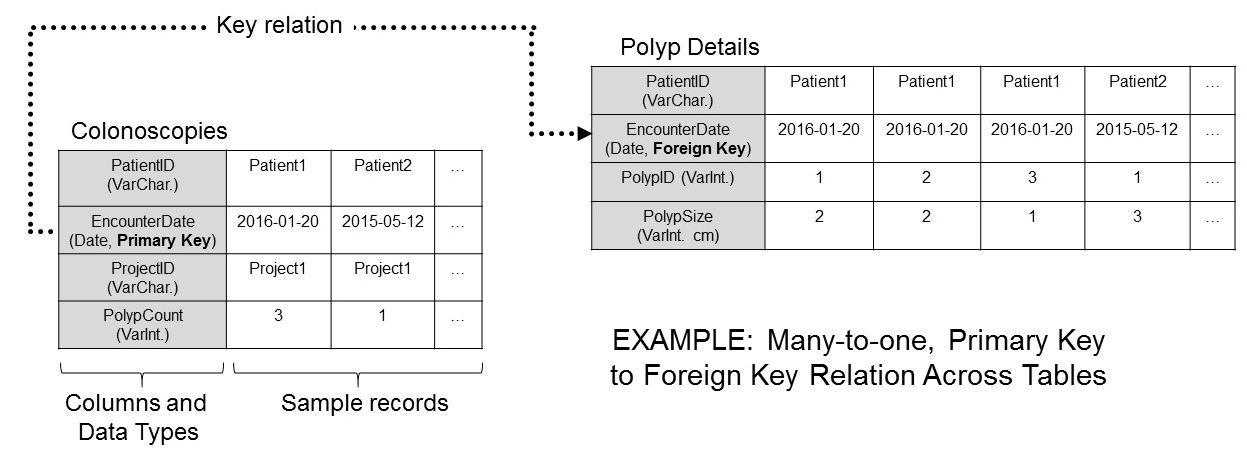
\includegraphics{keyrelation_clip.JPG}
\caption{Key relation, one-to-many on patientid across the Patients and
Colonoscopies tables.}
\end{figure}

\paragraph{Database Schema}\label{database-schema}

The schema refers to the design of tables and other schema objects,
including their relations to one another. This is the fundamental
structure and relations of the static data and database tables. The
generation of database schema is called normalization.

\begin{figure}[htbp]
\centering
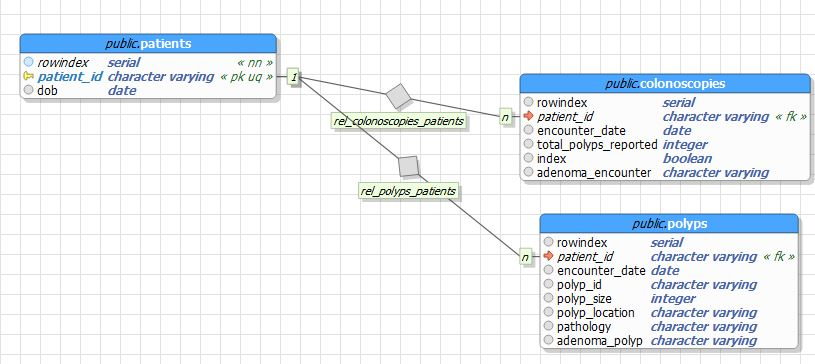
\includegraphics{patient_coln_polyps_tablerelations.jpg}
\caption{Database schema image created in pgModeler. Note the
primary-to-foreign key relations between patientid fields in the
Patients table and the Colonoscopies and Polyps tables, respectively.}
\end{figure}

The schema for the grady lab database will be backed up on the grady lab
\href{https://github.com/GradyLab/GradyLab_PostgreSQL}{github page}.

Database schema can be viewed as a series of table creation scripts
written in SQL. To automatically get table creation scripts from
pgAdmin, right click the table in the left-hand menu and select:
``Scripts'' \textgreater{} ``CREATE Script'' then save, or instead
select ``Backup'' and choose from the dump options tab whether to export
the schema, the data, or both.

\begin{figure}[htbp]
\centering
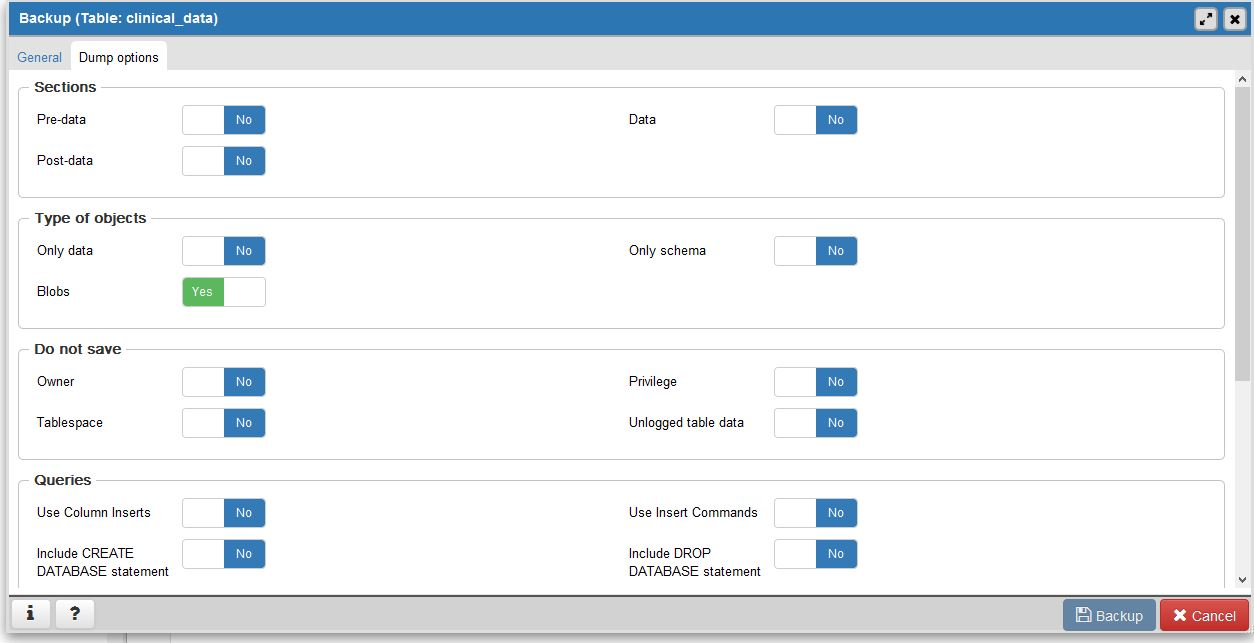
\includegraphics{backup_options.JPG}
\caption{Options for backing up a table schema and/or data in pgAdmin,
accessible from right-clicking the Table and selecting Backup.}
\end{figure}

\section{II. Practical Information}\label{ii.-practical-information-1}

\subsection{Setting Up The Connection (For Hutch
databases)}\label{setting-up-the-connection-for-hutch-databases}

The Hutch now hosts lab servers (or ``database containers'') on the
local gizmo clusters. These are then backed up periodically. MyDB
provides \href{https://mydb.fredhutch.org/doc_backup/}{restore
instructions}, and further updates to these details are expected soon.

\subsubsection{PostgreSQL Clients}\label{postgresql-clients}

\paragraph{Database Creation and Superuser
Access}\label{database-creation-and-superuser-access}

The following describes initial setup, with implicit superuser access
for the database creator. Skip further down for details on setting up
users with restricted access and logging in as such a user.

To connect to a database, first make sure a database container has been
created through Hutch \href{https://mydb.fredhutch.org/login}{MyDB}.
Store the user identification and password for later use, as you will
later connect to the server/container as a client with superuser access.

Next, install \href{https://www.postgresql.org/download/}{postgreSQL}
and \href{https://www.pgadmin.org/}{pgAdmin} to your local harddrive.
The former is the main system with certain essential modules and scripts
that extend functionality. The latter is a widely-used GUI for managing
postgreSQL databases, and includes highly useful options for data
viewing, import/export, management, etc. while conveniently displaying
underlying SQL code for user GUI interactions.

Set up a connection as a pgSQL client in pgAdmin by:\\
1. Right click `servers' in lefthand menu, then
Create\textgreater{}Servers\\
2. In popup window, select Connection tab\\
3. In connection tab, populate the entries with:\\
A. Host name (eg. ``mydb'')\\
B. Port (eg. 12345)\\
C. Maintenance Database (eg. ``name-of-database'')\\
D. Username\\
E. Password\\
4. Save.

You should have a connection to the database server hosted on the Hutch
gizmo clusters.

To start accessing databases, schemas, tables, etc. select the server
name then go to: Databases \textgreater{} select desired database
\textgreater{} Schemas \textgreater{} select desired schema or default
`public' schema \textgreater{} select/right-click Tables

\begin{figure}[htbp]
\centering
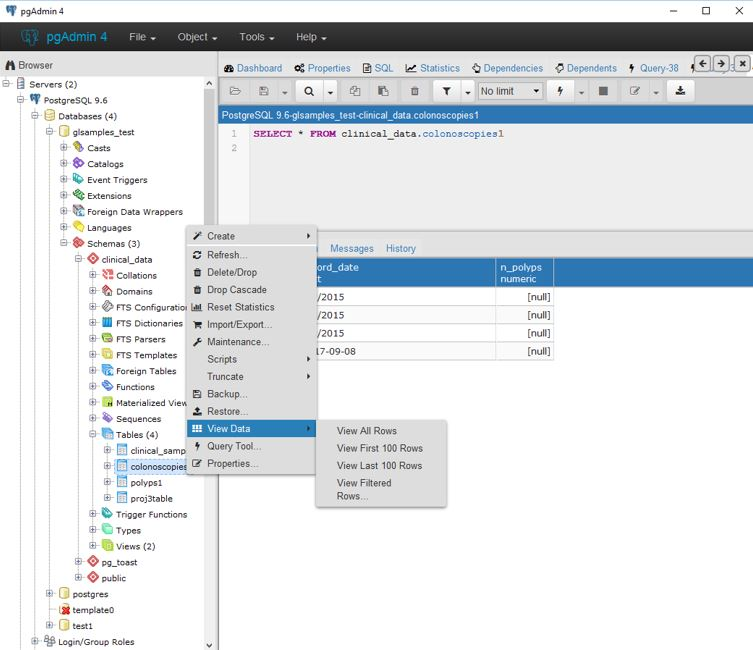
\includegraphics{pgadmin_scn.jpg}
\caption{Example pgAdmin view, navigating to and viewing entries in the
colonoscopies table. Note the SQL code above the table is the query
performed.}
\end{figure}

\paragraph{User Creation and Restricted
Access}\label{user-creation-and-restricted-access}

(TBD)

\subsection{Using pgAdmin to Manage
Data}\label{using-pgadmin-to-manage-data}

The following describes how to approach data management in the pgAdmin
GUI.

\subsubsection{Setting up the Binary
Path}\label{setting-up-the-binary-path}

Many essential features in pgAdmin require access to modules initially
installed with postgreSQL. To ensure pgAdmin can access these, Click
File\textgreater{}Preferences\textgreater{}Paths\textgreater{}Binary
Paths Enter the local path to the directory with the modules, eg. by
default: " C:\textgreater{}Program
Files\textgreater{}PostgreSQL\textgreater{}9.6\textgreater{}bin" Where
`\textgreater{}' is replaced by forward or backward slashes.

\subsubsection{Importing and Exporting Excel .csv
Files}\label{importing-and-exporting-excel-.csv-files}

Via pgAdmin, postgreSQL handles Excel quite well by default. Certain
variables are reformatted automatically, such as dates, when they are
imported. However, it should be possible to import a table with minimal
modification to the cell attributes in Excel. That is, on import the
Excel csv columns will be made to conform to the pre-specified column
attributes in the destination postgreSQL table.

That said, here are the general steps to take to import a csv from
Excel:\\
1. Either verify a postgreSQL table exists or make a new postgreSQL
table that will be the destination table for the Excel data. This will
involve specification of the column classes or data types, as well as a
specific name for each column and an explicit column order.

\begin{figure}[htbp]
\centering
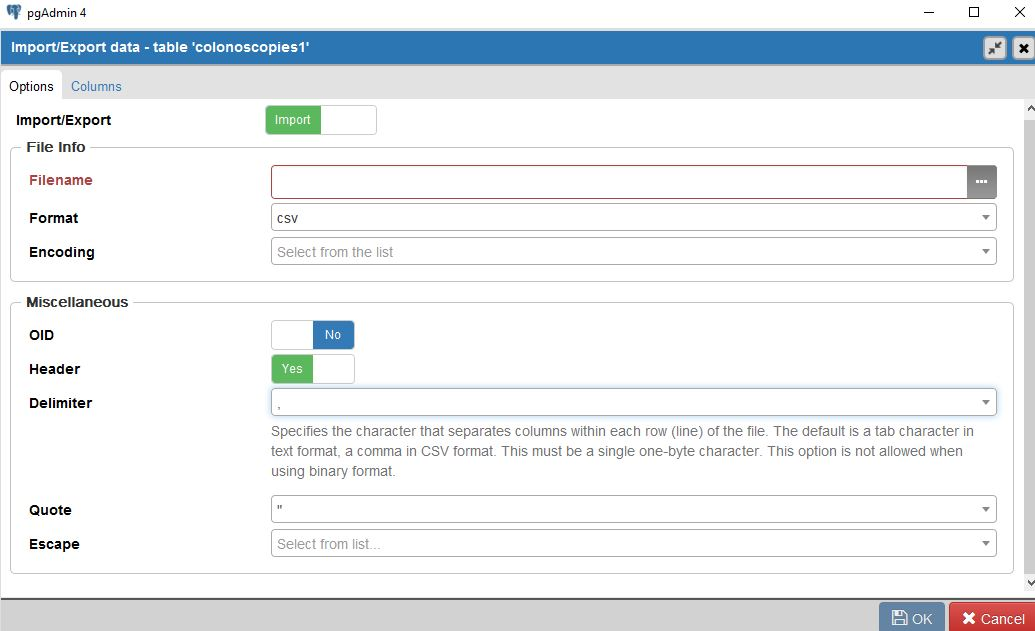
\includegraphics{csv_importoptions.jpg}
\caption{Setting config for importing Excel .csv files. Note that import
must be selected, format must be `.csv', header should be selected, and
delimiter must be changed to `,'. Finally, select only the columns in
the table using the Columns tab.}
\end{figure}

\begin{enumerate}
\def\labelenumi{\arabic{enumi}.}
\setcounter{enumi}{1}
\item
  Make sure the Excel file to import matches the format of the
  destination postgreSQL table. Namely, make sure:\\
  A. The excel file only contains columns corresponding to those in the
  destination table, B. All columns are in the same order as the
  destination table\\
  C. Data formatting doesn't violate any of the column class restraints
  in the destination table (eg. if a column is ``integer'' then no
  entries like ``123a'')
\item
  Once the csv is properly formatted, navigate to the table in pgAdmin,
  right click and select ``Import/Export''. On the window, select the
  parameters to match the Figure (Fig\#). Next, select the Columns tab
  and deselect all the columns except the ones in your excel file and
  destination table. The only columns left should correspond to your
  data columns, and these should be listed in the same order as in the
  csv and table.
\item
  Click `Ok.'
\end{enumerate}

\begin{figure}[htbp]
\centering
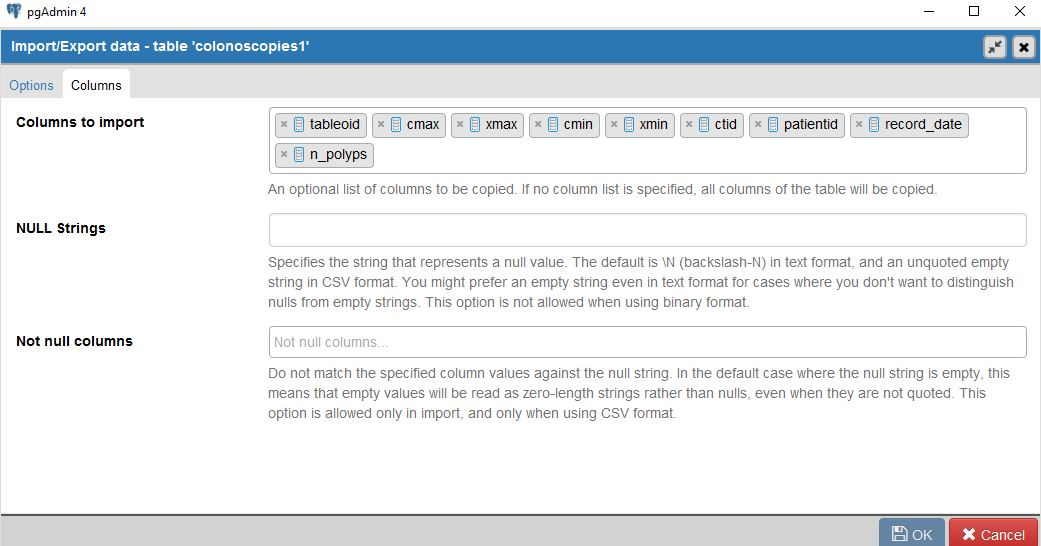
\includegraphics{csv_colselect.jpg}
\caption{Designating columns for the imported .csv file. Tableoid, cmax,
xmax, cmin, xmin, ctid, are examples of system-generated columns that
need to be removed before import.}
\end{figure}

\subsubsection{Views}\label{views}

Views are one primary way that such queries are possible in the
postgreSQL system. They are objects in the schema assembled by
``definitions'', which is essentially a SQL query or script. The
advantage of Views is they are dynamic. That is, when their referent
data is updated, they too can be rerun and updated to reflect those
changes. It is extremely convenient that the defining script is stored
with the pseudo-table, and therefore can be rerun as desired, even by a
user not versed in SQL.

The above leads to a need for iterative use and reuse of View definition
scripts. That is, to ensure efficient data storage and maximize utility,
scripts should be frames as generally as possible, such that the
filtering criteria can be modified without changing the underlying code
for the query.

For instace, one script might address the following query:

\textbf{``List all patients with at least two recorded colonoscopies,
where polyps were found on only the index, and whose age is at least 70
years old.''}

This should be translated to a View that filters on:\\
1. number of patient colonoscopies \textgreater{}=2;\\
2. number of polyps at index \textgreater{}0;\\
3. number of polyps at second (later) colonoscopy = 0;\\
and 4. age \textgreater{}= 70.

The specific qualifiers ``\textgreater{}=2'', ``\textgreater{}0'',
``0'', and ``\textgreater{}=70'' should thus be treated as variables
when writing the view definition, such that subsequent queries for 80
year old or 60 year olds with at least 3 colonoscopies or at least 1
polyp on followup could make use of the same or similar View definition,
with minimal alterations.

At a later date, these qualifiers could be treated as variables in a
wrapper function for a user interface (eg. a shiny application).

\section{III. Technical Information for Dynamic Data Access
Framework}\label{iii.-technical-information-for-dynamic-data-access-framework}

\subsection{Intro. to SQL}\label{intro.-to-sql}

(TBD)

Note: there are no inherent order to rows (aka. `tuples' or `records')
for data storage, and thus one needs to specify in SQL search if order
is important for query.

\subsection{Non-table Schema Objects}\label{non-table-schema-objects}

In addition to tables, there are several ephemera not related to static
stored data which are unique to object-relational management systems.
These include column indecies, views, and functions.

When dealing with rich datasets encompassing medical records, cohort
clinical data, lab sample records, and downstream analytical platform
records, framing a simple question can become complicated when
translated into a scripted query. This necessitates a well designed
static data storage layout that is conducive to these kinds of queries.

\subsection{View Design}\label{view-design}

Once a view has been effectively designed and saved, its definition can
then be copied and used iteratively with differing variable values.

When designing a view, it is helpful to break down the intended query
into subunits that can be tackled with their own code chunks. For
instance, to design a filter on age at colonoscopy, it is vital to first
derive the ages by taking the interval between the `dob' date of birth
provided in the patients table and the `encounter\_date' encounter date
provided in the colonoscopies table.

A second design strategy builds complex temporary tables through
nesting. While not necessarily aesthetically appealing, it ensures a
modular build where nested sub tables can be extracted, placed into a
view, and be used to successfully build a pseudo table with more limited
filtering criteria. An example is provided with 3b1 and 2b2 in the
appendix. 3b1 is a table showing encounters for patients whose index
encounters have a minimum number of total polyps reported by the
attending physician. 3b2 builds on this extensively by adding the
additional filtering criteria of minimum patient age at encounter,
minimum polyps reported at encounter, and minimum total encounters
available after filtering, while also adopting the index encounter polyp
count filter from 3b1.

\section{Appendix}\label{appendix}

\subsection{1. Common PGSQL/SQL
Commands}\label{common-pgsqlsql-commands}

\begin{enumerate}
\def\labelenumi{\arabic{enumi}.}
\tightlist
\item
  CREATE DATABASE - creates new database
\item
  CREATE INDEX - creates new index on a table column
\item
  CREATE SEQUENCE - creates new sequenc in existing database
\item
  CREATE TRIGGER - creates new trigger in existing database
\item
  CREATE VIEW - create new view in existing table
\item
  SELECT - retrieve records from a table
\item
  INSERT - adds one or more new records into table
\item
  UPDATE - modifies the data in existing table records
\item
  DELETE - removes existing records from a table
\item
  DROP DATABASE - destroys existing database
\item
  DROP INDEX - removes column index from an existing table
\item
  DROP SEQUENCE - destroys existing sequence generator
\item
  DROP TABLE - destroys existing table
\item
  DROP TRIGGER - destroys existing trigger
\item
  DROP VIEW - destroys an existing table view
\item
  CREATE USER - adds new postgreSQL account to the system
\item
  ALTER USER - modifies existing pgSQL user account
\item
  DROP USER - removes existing pgSQL user account
\item
  GRANT - grant rights on a database object to a user
\item
  REVOKE - deny rights on a database object from a user
\item
  CREATE FUNCTION - creats new SQL function within a database
\item
  CREATE LANGUAGE - creates new language definition within a database
\item
  CREATE OPERATOR - creates new SQL operator within a database
\item
  CREATE TYPE - creates new SQL data type within a database
\end{enumerate}

\subsection{3. Example View Definitions}\label{example-view-definitions}

\subsubsection{3a. QUERY: On a by-encounter,by-patient basis, how many
polyps have details recorded in the polyps
table?}\label{a.-query-on-a-by-encounterby-patient-basis-how-many-polyps-have-details-recorded-in-the-polyps-table}

Definition:

\begin{Shaded}
\begin{Highlighting}[]
\NormalTok{SELECT polyps1.encounter_date,}
    \KeywordTok{count}\NormalTok{(polyps1.encounter_date) AS count,}
    \NormalTok{polyps.patient_id}
   \NormalTok{FROM gldata.polyps}
\NormalTok{GROUP BY polyps.encounter_date, polyps.patient_id;}
\end{Highlighting}
\end{Shaded}

\subsubsection{3b1. What endoscopies are from patients whose index
endoscopy had a minimum number of polyps? This query is nested in
3b2}\label{b1.-what-endoscopies-are-from-patients-whose-index-endoscopy-had-a-minimum-number-of-polyps-this-query-is-nested-in-3b2}

Definition:

\begin{Shaded}
\begin{Highlighting}[]
\NormalTok{SELECT *}
\NormalTok{FROM gldata.colonoscopies AS coln}
\NormalTok{WHERE coln.patient_id }
\KeywordTok{IN} \NormalTok{(    SELECT colonoscopies.patient_id         }
            \NormalTok{FROM gldata.colonoscopies }
            \NormalTok{WHERE }\DataTypeTok{index=}\StringTok{'T'}
            \NormalTok{AND colonoscopies.total_polyps_reported >=}\StringTok{ }\DecValTok{1}\NormalTok{) /}\ErrorTok{*}\StringTok{ }\NormalTok{FILTER ON TOTAL POLYPS AT INDEX *}\ErrorTok{/}
\NormalTok{ORDER BY coln.patient_id,coln.encounter_date;}
\end{Highlighting}
\end{Shaded}

\subsubsection{3b. QUERY: What patients have encounters with a minimum
age, recorded polyp count, total polyp count, and minimum index
encounter polyp count? Show results as array aggregations by patient
(every row is a patient, entries can contain info from multiple
encounters).}\label{b.-query-what-patients-have-encounters-with-a-minimum-age-recorded-polyp-count-total-polyp-count-and-minimum-index-encounter-polyp-count-show-results-as-array-aggregations-by-patient-every-row-is-a-patient-entries-can-contain-info-from-multiple-encounters.}

Definition:

\begin{Shaded}
\begin{Highlighting}[]
\NormalTok{SELECT pat.patient_id,}
\NormalTok{t.ne AS num_encounters,}
\NormalTok{t.ed AS encounter_dates,}
\NormalTok{t.ea AS encounter_ages,}
\NormalTok{t.pr AS polyps_recorded_by_encounter,}
\NormalTok{t.tp AS total_polyps_reported,}
\NormalTok{t.i index_id}
\NormalTok{FROM gldata.patients pat,}
\NormalTok{( SELECT ct.patient_id,}
  \KeywordTok{array_agg}\NormalTok{(ct.age_yrs) AS ea,}
  \KeywordTok{array_agg}\NormalTok{(ct.encounter_date) AS ed,}
  \KeywordTok{array_agg}\NormalTok{(ct.npolyps) AS pr,}
  \KeywordTok{count}\NormalTok{(ct.encounter_date) AS ne,}
  \KeywordTok{array_agg}\NormalTok{(ct.total_polyps_reported) AS tp,}
  \KeywordTok{array_agg}\NormalTok{(ct.index) AS i}
  \KeywordTok{FROM} \NormalTok{( SELECT gc.patient_id,}
         \KeywordTok{date_part}\NormalTok{(}\StringTok{'year'}\NormalTok{, }\KeywordTok{age}\NormalTok{(gc.encounter_date, p.dob)) AS age_yrs,}
         \NormalTok{gc.encounter_date,}
         \NormalTok{gc.total_polyps_reported,}
         \NormalTok{gc.index,}
         \NormalTok{p.dob,}
         \NormalTok{npolt.n_polyps AS npolyps}
         \NormalTok{FROM gldata.patients AS p,}
         \NormalTok{gldata.colonoscopies AS gc,}
         \NormalTok{( SELECT glc.patient_id,}
           \NormalTok{glc.encounter_date,}
           \KeywordTok{count}\NormalTok{((polyps.encounter_date ||}\StringTok{ '-'}\NormalTok{) ||}\StringTok{ }\NormalTok{polyps.patient_id) AS n_polyps}
           \NormalTok{FROM gldata.colonoscopies glc}
           \NormalTok{LEFT JOIN gldata.polyps ON }\DataTypeTok{glc.patient_id =} \NormalTok{polyps.patient_id AND }\DataTypeTok{glc.encounter_date =} \NormalTok{polyps.encounter_date}
           \NormalTok{GROUP BY glc.patient_id, glc.encounter_date}
           \NormalTok{ORDER BY glc.patient_id, glc.encounter_date) npolt}
         \NormalTok{WHERE }\DataTypeTok{p.patient_id =} \NormalTok{gc.patient_id}
         \NormalTok{AND }\DataTypeTok{p.patient_id =} \NormalTok{npolt.patient_id }
         \NormalTok{AND }\DataTypeTok{gc.encounter_date =} \NormalTok{npolt.encounter_date }
         \KeywordTok{AND} \NormalTok{(gc.patient_id }\KeywordTok{IN} \NormalTok{( SELECT glc.patient_id}
                                       \NormalTok{FROM gldata.colonoscopies glc}
                                       \NormalTok{WHERE }\DataTypeTok{glc.index =} \NormalTok{true AND glc.total_polyps_reported >=}\StringTok{ }\DecValTok{0}\NormalTok{))) ct}
  \NormalTok{WHERE ct.age_yrs >=}\StringTok{ }\DecValTok{0} \NormalTok{AND ct.npolyps >=}\StringTok{ }\DecValTok{0}
  \NormalTok{GROUP BY ct.patient_id, ct.dob) t}
\NormalTok{WHERE pat.patient_id =}\StringTok{ }\NormalTok{t.patient_id}
\NormalTok{AND t.ne >=}\StringTok{ }\DecValTok{1}\NormalTok{;}
\end{Highlighting}
\end{Shaded}

\section{TODO}\label{todo-1}

\begin{enumerate}
\def\labelenumi{\arabic{enumi}.}
\tightlist
\item
  Add connections to pgsql example db and show results of View queries.
\item
  Add table export (to Excel .csv format) directions.
\item
  Flesh out the static repository structure plan, frame so updates are
  possible.
\item
  Flesh out Views script/query Appendix examples with known queries.
\end{enumerate}


\end{document}
